% equipose — The Mathematics of Posture-Angle Measurement
% Compile with: xelatex measurement_math.tex  (run twice for the TOC)
\documentclass[11pt]{article}

% ---- fonts (xelatex) -------------------------------------------------------
\usepackage{fontspec}
\setmonofont{Menlo}[Scale=0.92]
\newfontfamily\headingfont{Helvetica Neue}

% ---- math ------------------------------------------------------------------
\usepackage{amsmath}
\usepackage{amssymb}

% ---- layout ----------------------------------------------------------------
\usepackage[letterpaper,margin=1in]{geometry}
\usepackage{parskip}
\setlength{\emergencystretch}{2.5em}
\usepackage{array}
\usepackage{booktabs}
\usepackage{graphicx}
\usepackage{xcolor}
\usepackage{tikz}
\usetikzlibrary{angles,quotes,calc,positioning}
\usepackage{fancyhdr}

% ---- palette ---------------------------------------------------------------
\definecolor{ink}{HTML}{1F2933}
\definecolor{slate}{HTML}{52606D}
\definecolor{accent}{HTML}{0F766E}     % teal
\definecolor{accentbg}{HTML}{E6F3F1}
\definecolor{amber}{HTML}{B45309}
\definecolor{amberbg}{HTML}{FBF0DD}
\definecolor{rulec}{HTML}{CBD5E1}
\color{ink}

% ---- links (load late) -----------------------------------------------------
\usepackage{hyperref}
\hypersetup{
  colorlinks=true, linkcolor=accent, urlcolor=accent, citecolor=accent,
  pdftitle={equipose: The Mathematics of Posture-Angle Measurement},
  pdfauthor={ggmr}, pdfsubject={Pose-based posture angle measurement}
}

% ---- section styling (no titlesec available) -------------------------------
\makeatletter
\renewcommand\section{\@startsection{section}{1}{\z@}%
  {-3.25ex \@plus -1ex \@minus -.2ex}{1.3ex \@plus .2ex}%
  {\normalfont\Large\headingfont\bfseries\color{accent}}}
\renewcommand\subsection{\@startsection{subsection}{2}{\z@}%
  {-2.5ex \@plus -1ex \@minus -.2ex}{0.8ex \@plus .2ex}%
  {\normalfont\large\headingfont\bfseries\color{ink}}}
\makeatother

% ---- callout boxes (no framed/tcolorbox available) -------------------------
\newsavebox{\eqpbox}
\newenvironment{kbox}{%
  \par\smallskip\noindent
  \begin{lrbox}{\eqpbox}\begin{minipage}{\dimexpr\linewidth-2.2em\relax}\vspace{0.45em}}%
 {\vspace{0.45em}\end{minipage}\end{lrbox}%
  \noindent\colorbox{accentbg}{\hspace{0.3em}{\color{accent}\vrule width 2.6pt}\hspace{0.8em}\usebox{\eqpbox}\hspace{0.4em}}%
  \par\smallskip}
\newenvironment{cbox}{%
  \par\smallskip\noindent
  \begin{lrbox}{\eqpbox}\begin{minipage}{\dimexpr\linewidth-2.2em\relax}\vspace{0.45em}}%
 {\vspace{0.45em}\end{minipage}\end{lrbox}%
  \noindent\colorbox{amberbg}{\hspace{0.3em}{\color{amber}\vrule width 2.6pt}\hspace{0.8em}\usebox{\eqpbox}\hspace{0.4em}}%
  \par\smallskip}

% ---- header / footer -------------------------------------------------------
\pagestyle{fancy}\fancyhf{}
\renewcommand{\headrulewidth}{0.4pt}
\fancyhead[L]{\footnotesize\headingfont\color{slate}equipose}
\fancyhead[R]{\footnotesize\headingfont\color{slate}Measurement Mathematics}
\fancyfoot[C]{\footnotesize\color{slate}\thepage}

\newcommand{\figcap}[1]{\par\vspace{2pt}{\footnotesize\color{slate}\textit{#1}}\par}
\newcommand{\mname}[1]{\texttt{\small #1}}

\begin{document}

% ---- title block -----------------------------------------------------------
\thispagestyle{empty}
\noindent{\headingfont\color{ink}%
  {\fontsize{24}{28}\selectfont\bfseries equipose}\\[3pt]
  {\fontsize{15}{19}\selectfont\color{slate} The Mathematics of Posture-Angle Measurement}\par}
\vspace{5pt}
\noindent{\color{accent}\rule{\linewidth}{1.4pt}}
\vspace{4pt}
\noindent{\footnotesize\headingfont\color{slate}%
  AI Vision Posture Monitoring for Pediatric Hippotherapy (Cerebral Palsy)\quad\textbullet\quad ggmr\quad\textbullet\quad \today}
\vspace{14pt}

\noindent
This note documents exactly how \textbf{equipose} turns pose landmarks into the
posture angles it reports. Every value is computed in the \emph{two-dimensional
image plane} from the pixel coordinates of body landmarks; there is no depth or
3D reconstruction. Two small geometric primitives, a line-tilt and a three-point
joint angle, generate all eleven metrics. We give the precise formulas, a worked
numerical example, the per-frame to per-session aggregation, and the validity
conditions under which the numbers mean what they claim to.

\vspace{6pt}
{\color{rulec}\rule{\linewidth}{0.6pt}}
\setcounter{tocdepth}{2}
\tableofcontents
\vspace{2pt}
{\color{rulec}\rule{\linewidth}{0.6pt}}

% ===========================================================================
\section{The measurement model}

A pose backend (MediaPipe Pose, or MoveNet as a fallback) returns, for one
image, a set of named landmarks. Each landmark is a triple
\[
  \ell_i = (x_i,\; y_i,\; c_i), \qquad c_i \in [0,1],
\]
where $(x_i, y_i)$ are pixel coordinates and $c_i$ is the backend's
\emph{visibility / confidence}. The image origin is the \emph{top-left} corner
and the $y$-axis points \emph{downward}, the usual raster convention. Where
geometry only needs position we write a point as $a = (a_x, a_y)$ and drop the
confidence.

\begin{kbox}
\textbf{Two facts that shape everything below.}
\begin{enumerate}\setlength\itemsep{1pt}
  \item These are \emph{projective} angles measured in one camera's image plane.
        They approximate true anatomical angles only when the camera is
        perpendicular to the plane of interest (see \S\ref{sec:validity}).
  \item The confidence $c_i$ is the lever for occlusion: a metric is computed
        only when the landmarks it needs are confidently visible, otherwise it
        is skipped and flagged.
\end{enumerate}
\end{kbox}

% ===========================================================================
\section{Three geometric primitives}

Everything reduces to three pure functions of landmark coordinates.

\subsection{Line tilt: angle of a two-point line from an axis}

For two landmarks $a, b$ we measure the inclination of the line through them.
Because a tilt should not depend on which endpoint we list first, we fold the
raw angle into $[-90^\circ, +90^\circ]$:
\[
  \operatorname{wrap}_{90}(\phi) =
  \begin{cases}
    \phi - 180^\circ, & \phi > 90^\circ,\\[2pt]
    \phi + 180^\circ, & \phi < -90^\circ,\\[2pt]
    \phi, & \text{otherwise.}
  \end{cases}
\]

\begin{kbox}
\textbf{Tilt from horizontal} (\,$0^\circ$ = level\,) and \textbf{tilt from
vertical} (\,$0^\circ$ = plumb\,):
\begin{align*}
  \phi_{\mathrm H}(a,b) &= \operatorname{wrap}_{90}\!\big(\operatorname{atan2}(b_y - a_y,\; b_x - a_x)\big),\\[2pt]
  \phi_{\mathrm V}(a,b) &= \operatorname{wrap}_{90}\!\big(\operatorname{atan2}(b_x - a_x,\; b_y - a_y)\big).
\end{align*}
\end{kbox}

The swapped argument order in $\phi_{\mathrm V}$ measures from the vertical axis
instead of the horizontal. The sign encodes direction (because $y$ grows
downward, a positive $\phi_{\mathrm H}$ slopes down to the right).

\begin{center}
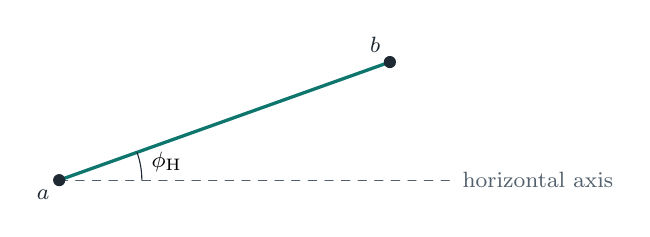
\begin{tikzpicture}[line cap=round]
  \coordinate (A) at (0,0);
  \coordinate (H) at (1.4,0);
  \coordinate (B) at (4.2,1.5);
  \draw[dashed,slate] (A) -- (5.0,0) node[right,slate,font=\footnotesize]{horizontal axis};
  \draw[very thick,accent] (A) -- (B);
  \fill[ink] (A) circle (2.2pt) node[below left,font=\footnotesize]{$a$};
  \fill[ink] (B) circle (2.2pt) node[above left,font=\footnotesize]{$b$};
  \pic["{\footnotesize$\phi_{\mathrm H}$}", draw=ink, angle radius=1.05cm, angle eccentricity=1.32]{angle=H--A--B};
\end{tikzpicture}
\figcap{Figure 1. Line tilt $\phi_{\mathrm H}(a,b)$: the angle of the landmark line above the horizontal.}
\end{center}

\subsection{Joint angle: the angle at a middle joint}

For three landmarks $a, m, b$ the angle \emph{at} $m$ is obtained from the dot
product of the two limb-segment vectors $u = a - m$ and $v = b - m$:

\begin{kbox}
\[
  \theta(a,m,b) \;=\; \arccos\!\left(\frac{(a-m)\cdot(b-m)}{\lVert a-m\rVert\,\lVert b-m\rVert}\right)
  \;\in\; [\,0^\circ,\,180^\circ\,].
\]
\end{kbox}

A straight limb gives $\theta = 180^\circ$; a right angle gives $90^\circ$.
The cosine argument is clamped to $[-1,1]$ for numerical safety, and a
degenerate (zero-length) segment returns $180^\circ$ by convention.

\begin{center}
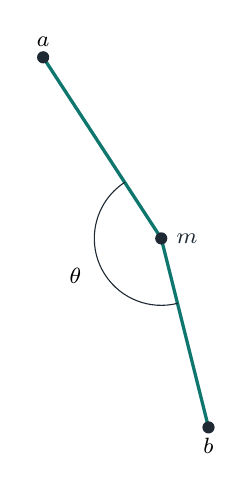
\begin{tikzpicture}[line cap=round]
  \coordinate (m) at (0,0);
  \coordinate (a) at (-1.5,2.3);
  \coordinate (b) at (0.6,-2.4);
  \draw[very thick,accent] (m) -- (a) node[above,font=\footnotesize,black]{$a$};
  \draw[very thick,accent] (m) -- (b) node[below,font=\footnotesize,black]{$b$};
  \fill[ink] (m) circle (2.2pt) node[right=2pt,font=\footnotesize]{$m$};
  \fill[ink] (a) circle (2.2pt);
  \fill[ink] (b) circle (2.2pt);
  \pic["{\footnotesize$\theta$}", draw=ink, angle radius=0.85cm, angle eccentricity=1.4]{angle=a--m--b};
\end{tikzpicture}
\figcap{Figure 2. Joint angle $\theta(a,m,b)$ at the vertex $m$, between segments $m{\to}a$ and $m{\to}b$.}
\end{center}

\subsection{Perpendicular distance: a point off an axis}

The signed-free distance from a point $p$ to the infinite line through $a$ and
$b$ (used for midline deviation):
\[
  d(p;a,b) \;=\; \frac{\big|(b_y-a_y)\,p_x - (b_x-a_x)\,p_y + b_x a_y - b_y a_x\big|}
                      {\sqrt{(b_y-a_y)^2 + (b_x-a_x)^2}}.
\]
Two convenience helpers complete the toolkit: the midpoint
$\operatorname{mid}(a,b) = \tfrac12(a+b)$ and the segment length
$\lVert a - b\rVert$ (used to normalize pixel distances by shoulder width).

% ===========================================================================
\section{The eleven posture metrics}

Each metric is one primitive applied to specific landmarks. Metrics split by
camera view, and by \emph{reliability}: \textbf{primary} metrics use
head / shoulder / trunk landmarks that stay visible above the saddle;
\textbf{best-effort} metrics use pelvis / hip / knee landmarks that the horse
and side-walkers frequently occlude.

\subsection{Front view (coronal plane)}

\begin{center}\small
\renewcommand{\arraystretch}{1.35}
\begin{tabular}{@{}>{\raggedright\arraybackslash}p{3.25cm} l >{\raggedright\arraybackslash}p{8.6cm}@{}}
\toprule
\textbf{Metric} & \textbf{Tier} & \textbf{Definition} \\ \midrule
\mname{head\_tilt}          & primary     & $\phi_{\mathrm H}(\ell_{\text{L ear}}, \ell_{\text{R ear}})$ \;(falls back to eyes) \\
\mname{shoulder\_tilt}      & primary     & $\phi_{\mathrm H}(\ell_{\text{L sh}}, \ell_{\text{R sh}})$ \\
\mname{pelvic\_obliquity}   & best-effort & $\phi_{\mathrm H}(\ell_{\text{L hip}}, \ell_{\text{R hip}})$ \\
\mname{trunk\_lateral\_lean}& primary     & $\phi_{\mathrm V}\!\big(\operatorname{mid}(\ell_{\text{L sh}},\ell_{\text{R sh}}),\, \operatorname{mid}(\ell_{\text{L hip}},\ell_{\text{R hip}})\big)$ \\
\mname{midline\_deviation}  & primary     & $\dfrac{d\big(\ell_{\text{nose}};\, \operatorname{mid}_{\text{sh}},\, \operatorname{mid}_{\text{hip}}\big)}{\lVert \ell_{\text{L sh}} - \ell_{\text{R sh}}\rVert}$ \;(fraction of shoulder width) \\
\mname{symmetry\_score}     & primary     & composite, see \S\ref{sec:composite} \\
\bottomrule
\end{tabular}
\end{center}

\subsection{Side view (sagittal plane)}

The camera-facing side $s \in \{\mathrm L, \mathrm R\}$ is chosen automatically as
the side with higher mean landmark confidence over a representative joint set
$J = \{\text{shoulder, hip, ear, knee, ankle}\}$:
\[
  s \;=\; \operatorname*{arg\,max}_{s \in \{\mathrm L,\mathrm R\}}\;
          \frac{1}{|J_s|}\sum_{j \in J_s} c_{j}.
\]

\begin{center}\small
\renewcommand{\arraystretch}{1.35}
\begin{tabular}{@{}>{\raggedright\arraybackslash}p{3.6cm} l >{\raggedright\arraybackslash}p{8.25cm}@{}}
\toprule
\textbf{Metric} & \textbf{Tier} & \textbf{Definition (side $s$)} \\ \midrule
\mname{forward\_trunk\_lean}     & primary     & $\phi_{\mathrm V}(\ell_{s,\text{sh}}, \ell_{s,\text{hip}})$ \;(falls back to ear$\to$shoulder) \\
\mname{neck\_forward\_angle}     & primary     & $\theta(\ell_{s,\text{ear}}, \ell_{s,\text{sh}}, \ell_{s,\text{hip}})$ \\
\mname{hip\_flexion}             & best-effort & $\theta(\ell_{s,\text{sh}}, \ell_{s,\text{hip}}, \ell_{s,\text{knee}})$ \\
\mname{knee\_angle}              & best-effort & $\theta(\ell_{s,\text{hip}}, \ell_{s,\text{knee}}, \ell_{s,\text{ankle}})$ \\
\mname{sitting\_alignment\_index}& primary     & composite, see \S\ref{sec:composite} \\
\bottomrule
\end{tabular}
\end{center}

\begin{center}
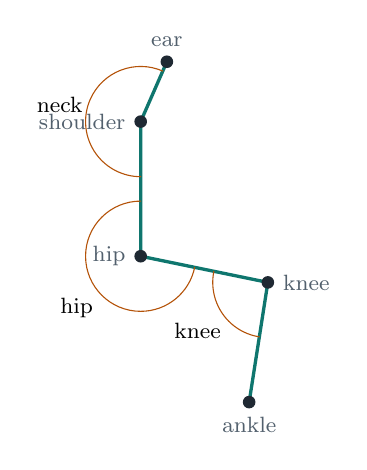
\begin{tikzpicture}[line cap=round,scale=0.95]
  \coordinate (ear) at (0.35,5.1);
  \coordinate (sh)  at (0.0,4.3);
  \coordinate (hip) at (0.0,2.5);
  \coordinate (knee) at (1.7,2.15);
  \coordinate (ank) at (1.45,0.55);
  \draw[very thick,accent] (ear)--(sh)--(hip)--(knee)--(ank);
  \foreach \p/\n/\pos in {ear/ear/above,sh/shoulder/left,hip/hip/left,knee/knee/right,ank/ankle/below}{
     \fill[ink] (\p) circle (2.4pt);
     \node[\pos=2pt,font=\footnotesize,slate] at (\p) {\n};
  }
  \pic["{\footnotesize neck}", draw=amber, angle radius=0.7cm, angle eccentricity=1.5]{angle=ear--sh--hip};
  \pic["{\footnotesize hip}", draw=amber, angle radius=0.7cm, angle eccentricity=1.5]{angle=sh--hip--knee};
  \pic["{\footnotesize knee}", draw=amber, angle radius=0.7cm, angle eccentricity=1.55]{angle=hip--knee--ank};
\end{tikzpicture}
\figcap{Figure 3. Sagittal landmark chain. \mname{neck\_forward\_angle}, \mname{hip\_flexion}, and \mname{knee\_angle} are the joint angles at shoulder, hip, and knee; \mname{forward\_trunk\_lean} is the tilt of the shoulder$\to$hip segment from vertical.}
\end{center}

\subsection{Composite indices}\label{sec:composite}

Two metrics summarize several others into a single $0$--$100$ score (higher is
better). They are deliberately simple weighted penalties; the scaling constants
are provisional and pinned for calibration at the pilot.
\begin{align*}
  \mname{symmetry\_score} &= \max\!\Big(0,\; 100 - \big(|\,\mname{head\_tilt}\,| + |\,\mname{shoulder\_tilt}\,| + 100\,|\,\mname{midline\_deviation}\,|\big)\Big),\\[3pt]
  \mname{sitting\_alignment\_index} &= \max\!\Big(0,\; 100 - \big(|\,\mname{forward\_trunk\_lean}\,| + |\,180^\circ - \mname{neck\_forward\_angle}\,|\big)\Big).
\end{align*}

% ===========================================================================
\section{Worked example}

Take three landmarks from a side view (pixels): ear $a=(90,80)$,
shoulder $m=(100,100)$, hip $b=(100,200)$. Then \mname{neck\_forward\_angle}
$= \theta(a,m,b)$:
\begin{align*}
  u = a-m &= (-10,\,-20), & v = b-m &= (0,\,100),\\
  u\cdot v &= (-10)(0) + (-20)(100) = -2000, &
  \lVert u\rVert &= \sqrt{500},\quad \lVert v\rVert = 100,\\
  \cos\theta &= \frac{-2000}{100\sqrt{500}} \approx -0.8944, &
  \theta &= \arccos(-0.8944) \approx 153.4^\circ.
\end{align*}
A forward-flexed neck (head dropping toward the chest) would pull this angle
\emph{down} from $180^\circ$; here $153^\circ$ reflects a mild forward lean. The
unit tests pin exactly these reference values.

% ===========================================================================
\section{From a measurement to a reported value}

\subsection{Confidence gating (occlusion handling)}
A metric is evaluated only when \emph{every} landmark it requires clears the
visibility threshold $\tau$ (default $\tau = 0.3$); otherwise its value for that
frame is undefined ($\varnothing$) and flagged. The reported per-metric
confidence is the minimum confidence over the landmarks used:
\[
  c_{\text{metric}} = \min_{j \in \text{used}} c_j, \qquad
  \text{value defined} \iff c_{\text{metric}} \ge \tau .
\]
This is why the lower-body, best-effort metrics legitimately drop out on a pony:
the saddle and side-walkers push hip / knee / ankle confidence below $\tau$.

\subsection{Temporal smoothing and aggregation (video)}
For a video, each metric yields a time series. Before aggregation the series is
passed through a \emph{One-Euro} filter to suppress per-frame jitter while
staying responsive; short gaps of missing frames are interpolated and long gaps
are preserved as $\varnothing$. Over the valid frames
$\mathcal V = \{\,t : v_t \neq \varnothing\,\}$ with acceptable range $[\,\ell, h\,]$:
\begin{align*}
  \bar v &= \frac{1}{|\mathcal V|}\sum_{t\in\mathcal V} v_t,
  & \sigma &= \sqrt{\frac{1}{|\mathcal V|}\sum_{t\in\mathcal V}(v_t-\bar v)^2},\\[3pt]
  p_{\text{in}} &= \frac{1}{|\mathcal V|}\sum_{t\in\mathcal V}\mathbf 1\!\left[\ell \le v_t \le h\right],
  & \delta_{\max} &= \max_{t\in\mathcal V}\,\max\!\big(0,\; \ell - v_t,\; v_t - h\big).
\end{align*}
Here $p_{\text{in}}$ is the fraction of the session spent inside the acceptable
range, and $\delta_{\max}$ is the worst excursion outside it.

\subsection{The single-photo case}
A photo is one frame, so $|\mathcal V| = 1$: there is no smoothing and no spread.
The aggregates collapse to
\[
  \bar v = v, \qquad \sigma = 0, \qquad p_{\text{in}} \in \{0, 1\},
\]
i.e.\ the reported value \emph{is} the single measurement and ``\,\% in range\,''
becomes a binary in/out flag. equipose therefore labels photo output a
\emph{snapshot}, not a trend.

% ===========================================================================
\section{Validity and limitations}\label{sec:validity}

\begin{cbox}
\textbf{These are 2D projective approximations, not goniometer readings.}
A single camera measures angles in its own image plane. The numbers approximate
the true 3D anatomical angles only when the optical axis is perpendicular to the
relevant plane: the \emph{front} camera for coronal tilts, the \emph{side}
camera for sagittal flexion. Any out-of-plane body rotation introduces error
that one view cannot recover.
\end{cbox}

Three practical consequences:
\begin{itemize}\setlength\itemsep{2pt}
  \item \textbf{Camera setup is part of the measurement.} Perpendicular optical
        axis, camera at the child's trunk height, full body in frame. These are
        prerequisites, documented in \texttt{SETUP\_PROTOCOL.md}.
  \item \textbf{Thresholds are placeholders.} The acceptable ranges
        $[\,\ell,h\,]$ behind every in/out flag, and the composite scaling
        constants, were not derived from clinical data. They are tunable
        defaults to be calibrated against clinician judgement at the pilot.
  \item \textbf{Lower-body metrics are best-effort by design.} On a pony the
        pelvis and legs are the most occluded and the most clinically
        interesting; equipose reports them when confident and abstains when not,
        rather than fabricating a number.
\end{itemize}

\vspace{8pt}
{\color{rulec}\rule{\linewidth}{0.6pt}}
\vspace{2pt}

\noindent{\footnotesize\color{slate}%
equipose is a research and screening aid, not a diagnostic device. Clinical
decisions remain with the therapist and physician. Source of truth for these
formulas: \mname{geometry.py}, \mname{angles\_front.py}, \mname{angles\_side.py},
and \mname{aggregate.py}.}

\end{document}
